\section{Configurable Systems}

%What is a Conf. system and why we use it
We call a system configurable if it offers options that allow developers and end-users to turn functionality on and off.
This gives the system the benefit of satisfying the demand of multiple user groups by providing a single software system containing various features
\cite{TooManyKnobs}.


\begin{figure}[h]
    \centering
    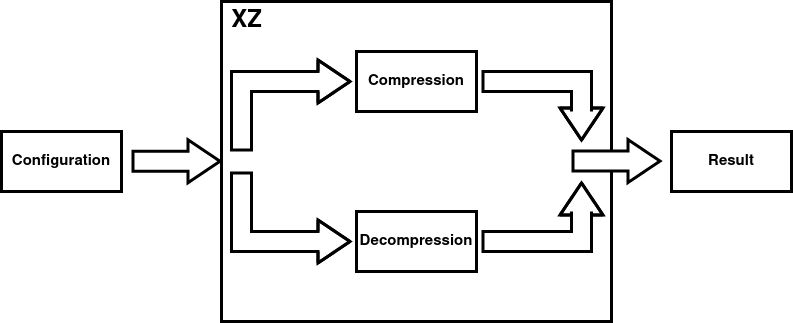
\includegraphics[scale=0.55]{gfx/ConfigurableSystemXZ.png}
    \caption{Simplified version of XZ.}
    \label{fig:xz}
\end{figure}

%Example for such a system using xz
As an example, let us inspect the compression tool \textsc{XZ}\footnote{Visited at 21.03.2023 \url{https://tukaani.org/xz/}}.
In \autoref{fig:xz} depicts a simplified version of \textsc{XZ}, which contains two main functions, encryption, and decryption. 
It is up to the user to decide what he needs, but regardless of his choice, a single software system contains both functions.